\documentclass[10pt,a4paper,oneside]{report}
%\usepackage[utf8]{inputenc}
\usepackage[a4paper,width=150mm,top=25mm,bottom=25mm]{geometry}
\usepackage{listing}
\usepackage{enumerate}
\usepackage{amsmath}
\usepackage{natbib}
\usepackage{amssymb, amsthm}
\usepackage{float}
%\usepackage{ dsfont }
\usepackage{amsfonts}
\usepackage{amssymb}
\usepackage{graphicx}
\graphicspath{{image/}}
\usepackage{times}
\usepackage{nomencl}
\usepackage{appendix}
\usepackage{setspace}
\usepackage{color}
\usepackage{fancybox}
\usepackage{lipsum}
\title{Double auction with regret}
		
\usepackage{fancyhdr}
\pagestyle{fancy}
\fancyhead{}
\fancyhead[RO,LE]{Double auction with regret}
\fancyfoot{}
\fancyfoot[LE,RO]{\thepage}
\fancyfoot[LO,CE]{Chapter \hspace{0.6mm}\thechapter}
\fancyfoot[CO,RE]{Govind}
\renewcommand{\headrulewidth}{0.4pt}
\renewcommand{\footrulewidth}{0.4pt}

%\usepackage[bookmarks=true]{hyperref}
%\usepackage{caption}
%\usepackage{subcaption}
%\usepackage[utf8]{inputenc}
%\usepackage{amsmath}
%\usepackage{amsfonts}
%\usepackage{amssymb}
%\usepackage{graphicx}
\date{}


%\fancyhf{}

%\fancyhead[RE]{\it{\nowuppercase{\leftmark}}}
%\fancyhead[LO]{\it{\nowuppercase{\rightmark}}}
%\fancyfoot[CE,CO]

\begin{document}
\begin{titlepage}
\begin{center}
%\vfill
	\vspace*{1cm}
	\Large
	A Report\\
	\vspace{0.5cm}
	\Large
	on\\
	\vspace{0.5cm}
	\Huge
	\textbf{"Finite Horizon Markov Decision Programs and Linear Programs"}\\
	\vspace{0.5cm}
	\vspace{1.5cm}
	\Large
	\textbf{Submitted in partial fulfillment of the requirements}\\
	\vspace{0.5cm}
	\Large
	of  the degree of\\
	\vspace{0.5cm}
	\Large
	\textbf{Master of Technology}\\
	\vspace{0.5cm}
	\Large
	by\\
	\vspace{0.2cm}
	\Large
	\textbf{(Gawas Prakash Arjun)}\\
	
	%\vspace{0.5cm}
	\Large
	(Roll no. 153190008)\\
	\vspace{0.5cm}
	\Large
	Supervised by\\
	\vspace{0.2cm}
	\Large
	\textbf{(Prof. Veeraruna Kavitha)}\\
	\textbf{(Prof. Ashutosh Mahajan)}\\
	\vspace{0.8cm}
	{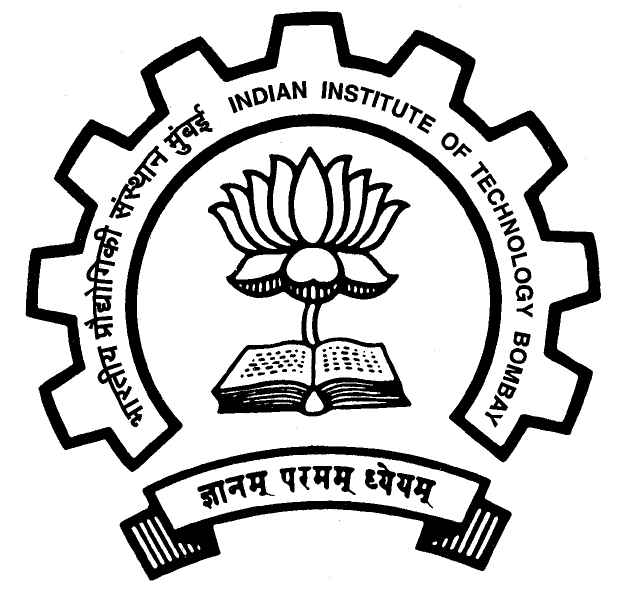
\includegraphics[scale=0.1]{logo.jpg}}\\
	\Large
	Inter-disciplinary program\\
	\Large
	in\\
	\Large
	Industrial Engineering and Operations Reserach (IEOR)\\
	\Large
	IIT BOMBAY\\
	\Large
		(2016-17)
\end{center}
\end{titlepage}
%\chapter*{Approval sheet}
%This is to certify that 
\chapter*{Declaration}
I declare that this written submission represents my idea in my own words and where other's idea or words have been included ,I have adequately cited and referenced the original source.I also declare that I have adhered to all principles of academic honesty and integrity and have not misrepresented or fabricated or falsified any/data/fact/source in my submission.I understand that any violation of the above will be cause for disciplinary action by the institute and can also evoke penal action from the sources which have thus not been properly cited or from whom proper permission has not been taken when needed.
\vspace{1cm}


\noindent Date:\hfill Govind Kumar Yadav                     
\begin{flushright}(153190002)\end{flushright}
\chapter*{Acknowledment}
I would like to extend thanks to the many people who so generously contributed to the work presented in the thesis.Special mention goes to my enthusiastic supervisor,\textbf{Prof. Mallikarjuna Rao} for giving me opportunity of working under his guidance.His Direction, motivation,affectionate guidance and support have been the source of inspiration to bring the report this shape.I thank all the other faculty member of Industrial Engineering And Operations Research, who made me realize the virtue of learning through sustained hard work.
\vspace{6mm}

\noindent I would like to thanks all those whose name i missed but have contributed in any form for building up of the thesis upto now.
\vspace{1cm}

\begin{flushright}
Govind Kumar Yadav\\
(153190002)
\end{flushright}

\chapter*{Abstract}
The project study is based on the \textbf{Regret management in double auction} which has been realised by the many online retailing service agencies.Despite promising functioning of the procedure, we still have a scope for some improvement in the process by incorporating some game theoretical approach into it.Reason for this involvement is that many customers do feel regret even they have successfully got their required product for any reason, so by virtue of this regret they might change their decision, even for the same situation next time in future.\vspace{6mm}

\noindent An attempt is made in this study to understand the regret related aspects in real life scenario.The study started with an objective of improving the quality transaction with the help of optimal strategies.After reviewing the relevant literature , customer behaviour and existing process flow in current scenario, implementation of regret aspects can be very useful tool in all double auction type of market.\vspace{6mm}

\noindent Several experiments are performed to find out the dominant strategies of all the agents in the market from game theoretical aspects,considering auction mechanism throughout the experiment.\vspace{6mm}

\noindent Some models have also be proposed in the report to explain the existence of regret in the market among the agents.This model also try to explain the implementation of double auction concept in any ordinary market.
\tableofcontents
\listoffigures
\listoftables
\chapter{Preamble}
\section{Introduction}
Bidders in first price sealed bid (FPSB) auction experiments overbid relative to the risk-neutral Nash equilibrium (RNNE), much as if they were risk averse, but there is a substantial amount of evidence that even if risk aversion is part of the explanation for overbidding, it is far from the complete explanation.\\
\noindent Thus the first effort in the  report is to find the reasonable answer which can explain the basic question that Why do we observe overbidding in first price sealed bid auction, this report will try to answer this question with theoretical as well as some experimental techniques. Before going into the details of the problem we would like to discuss some terminologies, which might be useful for understanding the discussion.\\
\noindent Even in the case of double auction there exists the scope of overbidding and underbidding by the players(buyers and sellers).\\
\noindent The double auction (DA). is one of the most common exchange institutions, used extensively in stock markets such as the New York Stock Exchange, commodity markets such as the Chicago Mercantile Exchange, and in markets for financial instruments, including options and futures\\
\noindent A brief description of regret, as a main reason for overbidding and underbidding behaviour will also be explained so as to see it other consequences in the future over the decision of the player.

\section{Scope of the project}
This project study is related to the bidding behaviour of the player (buyer or seller)under different scenarios.\\
\noindent Main interesting question will also be to find out the reason for overbidding or underbidding by the player for different types of auction.\\
\noindent The following specific tasks have been identified under the scope of this project:-
\begin{itemize}
\item Carry-out review of literature related to auction and regret mechanism.
\item Carry-out a detailed diagnostic study by several experiments to identify the main reason of change in bidding behaviour of the player under different scenario.
\item Conduct the regression analysis (method of least square) also, to find out the reason for overbidding in mainly first price auction (FPA).
\end{itemize}
\noindent The details of various studies carried out are reported in the subsequent chapters of this thesis,as mentioned in the below section.

\section{Outline of the report}
Project study presents the details of research carried out in a auction theory with involvement of regret parameter as a factor to observe overbidding in an auction.\\
\noindent \textbf{Chapter 1} deals with the introduction of basic mechanism of overbidding and underbidding observed in different auction.\\
\noindent Review of selected literature is done in \textbf{Chapter 2}.It presents the information regarding evolution of regret management in auction and factor affecting the effectiveness of it.So this chapter will cover all the literature details (basic terminologies,proof etc.,) required to understand the models in subsequent chapter.\\
\noindent \textbf{Chapter 3} will explain the models of chapter 2 using an experiment.Thus we argue that our model is capable of explaining the findings of our experimental results and thus can be generalised for all this kind of scenario existing in nature.\\
\noindent  Models and algorithm will be discussed thoroughly in \textbf{Chapter 4}.This models will be useful to understand the behaviour of the bidder in the market also the involvement of regret parameter is also considered in the model.\\
\noindent Further discussion over the regret parameter has been discussed in \textbf{Chapter 5} for many other existing types of auction in day to day life.\\
\noindent Now finally in \textbf{Chapter 6} we will discuss the conclusion of all literatures, models, algorithm and experiments discussed throughout the report.\\
\noindent We will also discuss the future work which might be interesting regarding the work initiated so for, along with the future scope of the models.

\chapter{Literature review}
\section{Introduction}
The main motive of the report is to find the reasonable answer which can explain the basic question that Why do we observe overbidding in first price sealed bid auction, this report will try to answer this question with theoretical as well as some experimental techniques. Before going into the details of the problem we would like to discuss some terminologies, which might be useful for understanding the discussion.
	\subsection{Basic terminology}
		\subsubsection{Auction}
		It is basically a price discovery mechanism by buying or selling goods or services by offering them up for bid, taking bids, and then selling the item to the highest bidder.

		\subsubsection{Risk Neutral Nash Equilibrium (RNNE)} It is the optimal bid submitted by the each bidder with the information of player's own valuation as well as the distribution of valuation of all other player also players does have any moral to change their decision based on possible regret , which might be felt in the future.

		\subsubsection{Risk aversion} Behaviour of humans (especially consumers and investors), when exposed to uncertainty, to attempt to reduce that uncertainty

		\subsubsection{Overbidding \& Underbidding}
 Process of submitting bid more than RNNE is overbidding and bidding less than RNNE is underbidding. 
		
		\subsubsection{Reservation price} It is a term referring to a limit on the price of a good or a service. On the demand side, it is the highest price that a buyer is willing to pay; on the supply side, it is the lowest price at which a seller is willing to sell a good or service. So reservation price is the minimum dollar amount that the owner of an item up for auction will accept as the winning bid in the auction. The reserve price prevents the auction from being won at a price that is lower than the item's owner will accept.

				\subsubsection{Auction as a game}
\begin{flushleft}
 \textbf{Player}: N potential bidders
	
	\textbf{Strategy set of players}: a set of non-negative bids

\textbf{Pay-off}: If players \textit{i} wins then pay-off $=$ \textbf{player's valuation – player's bid}, i.e., $V_i-b_i$
  			    
 
If players i lose then pay-off $=$ $0$ (player neither pay nor get anything)
\begin{equation*}   
\text{so, payoff} = 
\begin{cases}
V_i-b_i&,\text{If players \textit{i} wins}
\\
0  &,\text{otherwise}   

\end{cases}
\end{equation*}
  
  \textbf{Rule}:It depends on the types of auction
 \end{flushleft}
  		
  \subsubsection{Double Auction}
  A double auction is a process of buying and selling goods when potential buyers submit their bids and potential sellers simultaneously submit their ask prices to an auctioneer, and then an auctioneer chooses some price p that clears the market: all the sellers who asked less than p sell and all buyers who bid more than p buy at this price p. So any procedure in which buyers and sellers interact to arrange trade forms double auction.
  \begin{itemize}
 \item Contrast with the passive role of the seller in most auction models.
 \item Can be dynamic or one shot; most theory focuses on one-shot procedures, but most experimental work has focused on dynamic procedures
\end{itemize}  	       

\section{Theory}
William Vickrey derived risk neutral Nash equilibrium (RNNE) bidding behaviour in private value first price sealed bid auctions. However, bidding higher than the RNNE (overbidding) in first price private value auctions is one of the consistent and important findings of the experimental literature, which we would like to discuss throughout the report. So the main motive of this paper is that, in a game with incomplete information (e.g., auction), what seems the best action ex ante (before the information is revealed) may not turn out to be the best one ex post (after the information is revealed). This discrepancy may cause regret, and the decision maker reflects this regret concern in her decision if she can anticipate regret.

\subsubsection{Loser Regret}
Auctions are a good way to observe such discrepancies. For example, consider a first price private value auction in which a bidder values an object at \$1,000 and bids \$900. At the end of the auction, she learns that she lost because the highest bid was \$901. Bidding \$900 is not the best bid ex post because she could have won the
object in a profitable way by bidding \$902. In this situation, the fact that the ex ante best bid is no longer the best bid ex post will make her regret her ex ante decision. Since this regret may be felt only by the losing bidders, we will call it “ loser regret ”.

\subsubsection{Winner Regret}
The scenario above is not the only way that regret can be felt in an auction. Consider the scenario again, but this time after she bids \$900, the bidder learns not only that she is the highest bidder, but also that the second highest bid is \$50. Again, bidding \$900 is not the best bid ex post, e.g., she would still win with a bid of \$51 but pay less. Since this regret may be experienced only by the winner, we will call it “ winner regret ”.

\subsubsection{Regret Anticipation }
Now if the bidders know they are going to receive some feedback, they may anticipate regret. Intuitively, if the bidders anticipate that they are going to feel winner regret, they will decrease their bids. In contrast, if their anticipation is loser regret, they will overbid. First we theoretically show that these behaviours are observed in the equilibrium for risk neutral bidders with regret concerns. However, our theory is based on the assumption
that bidders do anticipate regret. For this clarification, we conduct experiments to answer whether they anticipate regret and, if so, whether they reflect it in their bids.

After above concepts a numbers of experiments were conducted to see if there is any change in the behaviour of the decision maker if he/she can anticipated regret and if, there is an effect then, which theory is responsible for this explanation. The most common explanation for the overbidding phenomenon in first price auctions is
risk aversion.

\subsubsection{flow of the problem}
We have divided the whole discussion into the four section .In Section I, we characterize the symmetric equilibrium bidding strategy under loser and winner regret in first price sealed bid auctions. In Section II, we conduct an experiment to check if bidders change their strategies in a first price auction depending on the information that can potentially make them anticipate regret. In Section III, we argue that our model is capable of explaining the findings of our experimental results. In Section IV, in order to check how introducing regret perturbs the revenue equivalence theorem, we consider other well-known auctions, namely second
price, English, and Dutch auctions. Section V concludes the overall discussion.

\noindent Before actually going to the model part, let us find out the Risk neutral Nash equilibrium (RNNE).
Let $V_i$ be the valuation of the player \textit{i}, and each valuation $V_j\sim$ U[0,100] where \textit{j} is any player out of N
  \begin{flushleft}
 where,$b_i$ be the bid submitted by player \textit{i}
       Bid of any player \textit{j} is given by 
       \end{flushleft}
       \begin{equation*}       
     b_j = f(V_j) = c\times(V_j)       
       \end{equation*}
    \begin{flushright}
    where,$c\in [-1,1]$ 
    \end{flushright}
    the expected utility of the player i is given by, 
\begin{align}
\nonumber
\text{expected payoff} &= (V_i-b_i)\times Prob(\max_{j\neq i}cV_j < b_i)\\
\nonumber
&= (V_i-b_i)\times (\frac{b}{100c})^{N-1}
\end{align}	
Now optimal bid for player i (RNNE) is given by solving below optimization problem for $b_i$ , given as:
\begin{equation*}
\max_{b_i>0}(V_i-b_i)\times(\frac{b}{100c})^{N-1}
\end{equation*}
\begin{equation*}
So,b_i = \big(\frac{N-1}{N}\big)V_i
\end{equation*}
\citep{dong2014double} \textbf{Hence,Optimal bid in FP auction under risk neutral condition (i.e., RNNE) is {$\big(\frac{N-1}{N}\big)V_i$}}

\subsubsection{Economic analysis of double auction}
From an economist's perspective, the interesting problem is to find a competitive equilibrium - a situation in which the supply equals the demand.

In the simple bilateral trade scenario, if $B \geq S$ then any price in the range [S,B] is an equilibrium price, since both the supply and the demand equal 1. Any price below S is not an equilibrium price since there is an excess demand, and any price above B is not an equilibrium price since there is an excess supply. When $B<S$, any price in the range (B,S) is an equilibrium price, since both the supply and the demand equal 0 (the price is too high for the buyer and too low for the seller).

In a more general double auction, in which there are many sellers each of whom holds a single unit and many buyers each of whom wants a single unit, an equilibrium price can be found using the natural ordering of the buyers and sellers:
\textbf{Natural ordering}:
\begin{enumerate}
\item[\textbf{•}] Order the buyers in decreasing order of their bid: $b_1\geq b_2\geq...\geq b_n$
\item[\textbf{•}] Order the sellers in increasing order of their ask: $s_1\leq s2\leq...\leq s_n$
\item[\textbf{•}] Let k be the largest index such that $b_k\geq s_k$ (the "break-even index").
\end{enumerate}

\citep{gjerstad1998price} Every price in the range [$max(s_k,b_{k+1}),min(b_k,s_{k+1})$] is an equilibrium price, since both demand and supply are k. It is easier to see this by considering the range of equilibrium prices in each of the 4 possible cases (note that by definition of k, $b_k+1 < s_{k+1}$):\\
\begin{table}[h]
\centering
\begin{tabular}{|c|c|c|}\hline
& $s_{k+1} > b_k $	& $s_{k+1}\leq b_k $\\ \hline
$b_{k+1} < s_k	$& $[s_k,b_k]$	&$[s_k,s_{k+1}]$\\ \hline
$b_{k+1} \geq s_k$& $[b_{k+1},b_k]$&$[b_{k+1},s_{k+1}]$\\ \hline

\end{tabular}
\end{table}
\section{Model Part}
In this we will try to see the change in form of utility under loser and winner regret condition and also the overbid and underbid, theoretically

\noindent Let There is only a single item for sell, and there are N potential bidders. $V_i$ (valuation of player \textit{i}) is independently and identically drawn from an uniform random variable between $[\underline{V},\overline{V}]$ according to an increasing distribution function F, and f is the density function corresponding to F. Without loss of generality,
\textbf{Assume that the reservation price of the seller is zero.}

\noindent Suppose the seller sells the object by a first price sealed bid auction (FP), i.e., the participants submit their bids simultaneously in sealed envelopes and the highest bidder gets the object at the price he/she offered by his/her bid. Assume that any tie is broken by assigning the object to one of the highest bidders, randomly.

\subsection{Loser Regret in First price sealed bid aution}
Suppose, at the end of FP, the bidders learn not only their winning/losing position but also, if they lose, they learn the winning bid. The utility of a losing bidder depends on the regret she feels. If the winning bid is less than the valuation of a losing bidder, then the ex post best action for this bidder is bidding a little more than the winning bid. Therefore, loser regret is defined as a function of the difference between her valuation and the winning bid if the winning bid is affordable.

\noindent So there will be change in the form of utility, as shown below:\citep{filizy2005auctions}
\begin{equation*}
U_i(V_i,b_i/b^w) =  
\begin{cases}
V_i-b_i &,\text{if \textit{i} wins}
\\
-g(V_i-b^w)&,\text{if \textit{i} lose}	
\end{cases}
\end{equation*}
Where $b^w$ is the highest bid (the bid of the winner), and g(.): $\mathds{R} \to \mathds{R}_+$ is the loser regret function which is assumed to be non-negative, non-decreasing, and differentiable. The bigger the difference between her value and the winning bid, the more a bidder may feel loser regret.

\noindent \textbf{Note:} Moreover, assume g(x) = 0 for all $x \leq 0$ ,because if a bidder loses and learns that the winning bid is not affordable to her, i.e., $V_i\leq b^w$ then there is no reason for loser regret. In other words, even if she has bid more than the winning bid, she would not have made positive profit because that bid would have been more than her valuation

\noindent Intuitively, since in our model the bidders who did not get the object may re-evaluate their bids by considering the winning bid, and some of them may regret their too low bids, by anticipating the regret possibility, they may end up bidding more than the traditional case, i.e., overbidding may be observed if the bidders are motivated by loser regret.\citep{filizy2005auctions}
\subsubsection{Theorem 1}
In a first price sealed bid auction with loser regret, the symmetric equilibrium bidding strategy $(b^{{FP}_{lr}}(.)):[\underline{V} , \overline{V}] \to [0, \infty))$ must satisfy the following condition:\citep{filizy2005auctions}
\begin{equation}
E_X[X|X<V] = b^{{FP}_{lr}}(V)- E_X[g(X-b^{{FP}_{lr}}(X))|X<V],
\end{equation}
Where X is the highest of N-1 values.

\begin{flushleft}
\textbf{Remark 1:} The left-hand side of equation (1) is the actual symmetric equilibrium strategy in a first price auction in the standard theory. Hence, in FP with loser regret, the symmetric equilibrium strategy is higher than standard theory suggests,i.e., $b^{{FP}_{lr}}(V)\geq b^{{FP}}(V)$  $\forall  V\in [\underline{V},\overline{V}]$ since g(.)is assumed to be non-negative.
\end{flushleft}

\begin{flushleft}
\textbf{Remark 2:} Loser regret concerns of bidder's increase the seller's expected revenue in FP since the equilibrium bidding strategy will be higher, as explained in Remark 1.

\subsection{Winner Regret in First price sealed bid auction}
Suppose at the end of the auction, bidders know not only their winning/losing position but also, if they win, the submitted second highest bid. Winner regret is a function of the difference between actual payment (her bid) and the minimum amount that would preserve her winning position after she learned the other bids. Formally, the utility function of bidder i, with valuation $v_i$ and bid $b_i$, in first price sealed bid auction takes the following form:\citep{filizy2005auctions}
\begin{equation*}
U_i(V_i,b_i/b^2) =  
\begin{cases}
V_i-b_i-h(b_i-b^2) &,\text{if \textit{i} wins}
\\
0&,\text{if \textit{i} lose}	
\end{cases}
\end{equation*}
Where $b^2$ is the highest bid (the bid of the winner), and g(.): $\mathds{R}_+ \to \mathds{R}_+$ is the winner regret function.If a bidder wins the object with a tie, then ex post she may not feel any regret because by bidding any smaller amount she would lose, or by bidding any bigger amount she would pay more, so assume h(0) = 0. The bigger the discrepancy between the actual bid and the ex post best bid is, the more regret may be felt; therefore, assume h is a non-decreasing function. Since the winner's monetary pay-off is shaded by regret, we should expect, in equilibrium, lower bids than those in traditional risk neutral case.Knowing that some ex post regret may be experienced, individuals may be afraid of bidding too aggressively.

\subsubsection{Theorem 2}
In a first price sealed bid auction with winner regret, the symmetric equilibrium bidding strategy $(b^{{FP}_{wr}}(.)):[\underline{V} , \overline{V}] \to [0, \infty))$ must satisfy the following condition:\citep{filizy2005auctions}
\begin{equation}
E_X[X|X<V] = b^{{FP}_{wr}}(V)+ E_X[h(b^{{FP}_{wr}}(V)-b^{{FP}_{wr}}(X))|X<V],
\end{equation}
Where X is the highest of N-1 values.

\begin{flushleft}
\textbf{Remark 3:} The left-hand side of equation (2) is the symmetric equilibrium strategy (RNNE)
in a first price auction in the traditional theory. Hence, in a first price sealed bid auction with winner regret, the symmetric equilibrium strategy is less than the RNNE, i.e., $b^{{FP}_{wr}}(V)\geq b^{{FP}}(V)$  $\forall  V\in [\underline{V},\overline{V}]$ since h(.)is assumed to be non-negative.
\end{flushleft}
\begin{flushleft}
\textbf{Remark 4:}Winner regret concerns of bidders decrease the seller’s expected revenue in FP since the equilibrium bidding strategy will be lower, as explained in Remark 3
\end{flushleft}
\end{flushleft}

\subsection{Game-theoretic analysis in double auction}
A double auction can be analysed as a game. Players are buyers and sellers. Their strategies are bids for buyers and ask prices for sellers (that depend on the valuations of buyers and sellers). Pay-offs depend on the price of the transaction (determined by the auctioneer) and the valuation of a player. The interesting problem is to find a Nash equilibrium - a situation in which no trader has an incentive to unilaterally change their bid/ask price.\\
\noindent Consider the bilateral trade scenario, in which the buyer submits a bid of b and the seller submits s.\\
\noindent Suppose an auctioneer sets the price in the following way:\citep{dong2014double}
\begin{enumerate}
\item[\textbf{•}] If $s>b$ then no trade occurs (the seller wants more than the buyer pays)
\item[\textbf{•}] $ s\leq b$ then $p=(b+s)/2$
\end{enumerate}
 
 \begin{equation*}
 \text{Now, the utility of the buyer =}
 \begin{cases}
 0,& \text{if $s>b$};\\
 B-p,&\text {if $s\leq b$} 
 \end{cases}
 \end{equation*}
	\begin{flushright}
	where B is the true value of the buyer)\end{flushright}
	\begin{equation*}
 \text{And,the utility of the seller =}
 \begin{cases}
 0,& \text{if $s>b$};\\
 p-S,&\text {if $s\leq b$} 
 \end{cases}
 \end{equation*}
	\begin{flushright}
	where S is the true value of the seller)\end{flushright}
In a complete information (symmetric information) case when the valuations are common knowledge, it can be shown that the continuum of pure strategy efficient Nash equilibriums exists with ${\displaystyle b=s=p\in [B,S].}$ This means that, if $B>S$, there will be no equilibrium in which both players declare their true values: either the buyer will be able to gain by declaring a lower value, or the seller will be able to gain by declaring a higher value.

\chapter{Experimental review}
\section{Introduction}
We showed that winner regret and loser regret have different implications for the equilibrium bidding strategies. In FP, winner regret concern leads to underbidding, whereas loser regret concern leads to overbidding compared to the RNNE.

\noindent Now, the natural question is whether the bidders anticipate any form of regret and reflect this concern in their bids. In order to answer this question, we conduct an FP experiment under different information structures, so that either form of regret might be anticipated.

\noindent We created three conditions that differ only in terms of information structures. In the \textbf{no feedback condition}, bidders will not learn anything about other's bids; \textbf{in the winner regret condition}, the winner will learn the second highest bid but the losers will not learn anything; and in the \textbf{loser regret condition}, the losers will learn the winning bid, but the winner will not learn anything.\citep{filizy2005auctions}

\begin{enumerate}

\item[\textbf{1.}] We want to conduct an experiment to see whether individuals reflect their concern of regret in their bidding strategies, not to see what they feel after the auction. It is hypothesized that the bids in the loser regret condition will be higher than those in the no feedback condition, and the bids in the winner regret condition will be lower than those in the no feedback condition.
\item[\textbf{2.}] Regret is a feeling one might experience after the action is taken and the uncertainty of the foregone actions is also resolved. Therefore, someone facing the same decision in a repeated fashion might reflect the regret of the previous round on the decision of the next round.\cite{bell1982regret}
\begin{enumerate}
\item[\textbf{a.}] Our theory relies, however, on the fact that bidders anticipate the future regret and they take this into account in their current decisions. To avoid this history-dependent regret explanation, unlike the standard lab auction experiments, we conduct a one-shot auction experiment.

\item[\textbf{b.}]In order to have more than one data point from each subject in a one-shot auction experiment, we propose a variation of the strategy method, which we call the \textbf{“bid on list method.”} In this method, each subject reports bids for several different valuations.	
\end{enumerate}
\end{enumerate}

\section{Description of the experiment (Method)}	
The experiment involved six sessions. In each session, one of the three conditions was administered. The numbers of participants in condition 1, 2, and 3 were 28, 32, and 36, respectively. No subject participated in more than one session.\citep{filizy2005auctions}

\noindent In our auction experiment, we created groups of four bidders and gave each of them a list of ten possible valuations. Different lists were given to each of the four bidders, but the same lists were used for each group. Each number on each list was drawn uniformly and independently between 0 and 100, rounded to the nearest cent, and this was common knowledge for the participants. Additionally, the participants were informed that only one of those ten numbers in their lists was their correct value, but they did not know which one. They needed to bid for every value they saw in the list as if it were the correct valuation of the object for them. The participants were told that after everyone submitted their bids, one valuation would be randomly selected and this would determine the relevant value and bid for each of them. The bidder who had submitted the highest bid for the selected row of the list won the fictitious good at the price of her bid, and she was paid in experimental dollars the difference between her valuation and her bid.\citep{filizy2005auctions}

\noindent Each group of four bidders was assigned to one of the three different conditions. Their condition was indicated on a separate page in the instructions in order to make sure they read this part of the instructions. The conditions were as follows:\citep{filizy2005auctions}

\noindent \textbf{Condition 1(No feedback):}Participants were told before they bid that, at the end of the auction, they were going to learn if they won or not, and no additional information would be given.

\noindent \textbf{Condition 2(Winner regret):}Participants were told before they bid that, at the end of the auction, they were going to learn if they won or not, and if they won, they would also learn the second highest bid that had been submitted.

\noindent \textbf{Condition 3(Lose regret):}Participants were told before they bid that, at the end of the auction, they were going to learn if they won or not, and if they did not win, they would also learn the highest bid that had been submitted.

\noindent After each participant had submitted their lists of bids, and before determining their true valuations, a survey was administered. In this survey, we listed a set of emotions and asked the subjects to rate the intensity of emotions that they felt after they received the relevant information. The ratings were between 1 and 9, where 1 indicated “not at all” and 9 indicated “very much.”

\subsection{Result}
For each condition, the averages of the bids corresponding to the same valuations were calculated. Figure 1 plots the average bids for the corresponding valuations for no feedback, winner regret, and loser regret. The linear estimation of plotted points of each condition is drawn in the same figure  \ref{fig:x graph}.\citep{filizy2005auctions}
\begin{figure}[H]
\centering
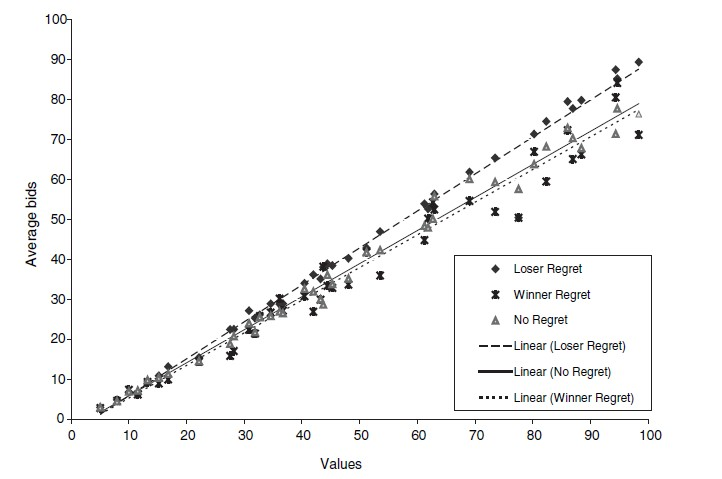
\includegraphics[scale=0.64]{t2.jpg}
\caption{The Average Bids for the Corresponding Valuations for No Feedback,Winner Regret, and Loser Regret Conditions \citep{filizy2005auctions}}
\label{fig:x graph}
\end{figure}



\noindent The slope of the linear estimation (passing through zero) of the \textbf{average bids under loser regret is 0.87} from table \ref{fig:t1}, which is \textbf{significantly higher} than that \textbf{under winner regret}, which is \textbf{0.77}, since the \textbf{95 percent confidence intervals} of each estimate do not overlap. Similarly, the slope of the linear estimation (passing through zero) of the average bids under no feedback is significantly lower than that under loser regret, since the \textbf{95 percent confidence intervals} of each estimate do not overlap. There is no significant difference, however, between the no feedback and winner regret conditions\citep{filizy2005auctions}.\\[0.6mm]

\begin{table}[H]
\centering
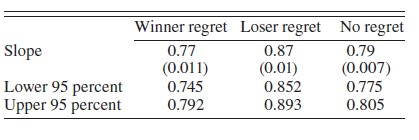
\includegraphics[scale=0.9]{t1.jpg}
\caption{Linear Estimation of Bidding Strategies Under Each Condition \citep{filizy2005auctions}}
\label{fig:t1}
\end{table}

Additionally, the averages of the emotions under each condition are summarized in Table \ref{fig:t2}. A t-test on the survey data suggests that the average intensity of regret under loser regret is significantly higher than that under winner regret (t = 6.2548, $P<0.01$)\citep{filizy2005auctions}.
\begin{table}[H]
\centering
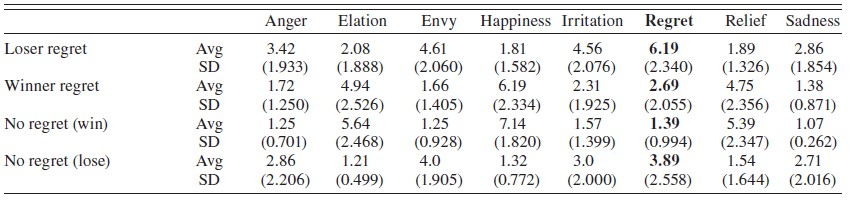
\includegraphics[scale=0.50]{t3.jpg}
\caption{Average and standard deviation of the intensities of emotions under each condition \citep{filizy2005auctions}}
\label{fig:t2}
\end{table}

\noindent \textbf{Note:} 	From table \ref{fig:t2} we can see that emotion associated with regret, under loser regret is quite high, thus 	bidder gets influenced by the fear of going through loser regret in future than all other regret.\\[2 mm]

\noindent In order to tell more about individual bidding behaviour, we define a typical variable for each individual to measure how she shades her value while bidding. To generate this variable for a given subject, first we calculated \textbf{the bid/value ratios} for the subject’s bid-value pair and then take the average of these ratios. We call this variable the individual bid/value coefficient
This bid/value coefficient is a useful tool to see the impact of valuation on the thinking of a bidder while bidding for each valuation.

\begin{figure}[H]
\centering
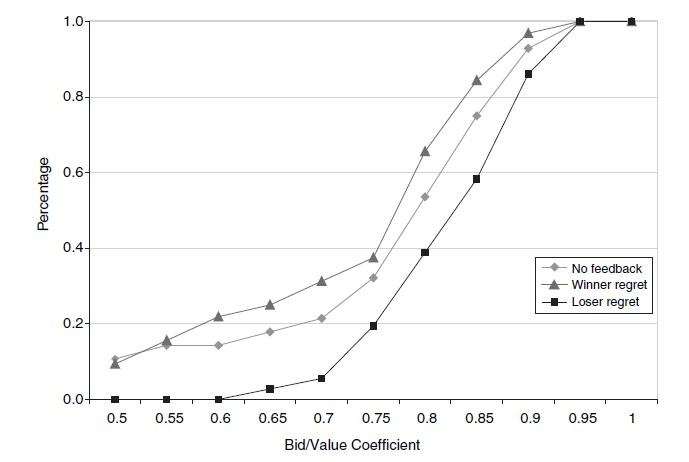
\includegraphics[scale=0.7]{t4.jpg}
\caption{CDFs of Individual Bid/Value Coefficients \citep{filizy2005auctions}}
\label{fig:f2}
\end{figure}

\noindent Figure \ref{fig:f2} demonstrates the cumulative distribution functions (CDFs) of individual bid/value coefficients under winner and loser regret conditions. First observe that there is a first-order stochastic domination between the CDFs. This domination indicates that the individual- level data still have the property that under the loser regret treatment the bid/value coefficients are higher than the winner regret coefficients.\\
\noindent It can be seen from the Figure \ref{fig:f2} that in the winner regret condition, 31 percent of the subjects have bid/value coefficients below 0.7. In the loser regret condition, however, this percentage is 5. This means that the loser regret condition made most of the subjects bid aggressively. Additionally, these coefficients are dense around the estimated slope of the bidding function (0.87) for the loser regret condition (80 percent of the subjects have coefficients between 0.75 and 0.95). On the other hand, the winner regret condition did not affect the bids of the subjects in a clear way. The bid/value coefficients in this group vary quite a bit.

\section{Experimental Results with Theory}
In this section, we will try to explain these experimental results using our theory. For this, we need to determine the RNNE for FP in the traditional theory and use it as a benchmark to detect overbidding/underbidding behaviour if there is any.\\
\noindent The RNNE of a bidder with valuation V is the expected second highest valuation, given that V is the highest, i.e.,$b^{\ast}(V)= E_X[X|X<V]= {\big(\frac{N-1}{N}\big)V_i}$.

\noindent In our setting with four bidders whose valuations are drawn from distribution $\sim U[0,100]$, this equilibrium bidding strategy corresponds to $b^{\ast}(V)= 0.75V$

\noindent In the loser regret condition, the estimated bidding strategy is $\hat{b}^{{FP}_{lr}}=0.87V$, which is significantly above the RNNE bidding strategy. This is in line with our theoretical predictions (see Remark 1). In the winner regret condition, however, the estimated bidding strategy is 
$\hat{V}^{{FP}_{wr}}=0.77V$,which is not significantly different from what the RNNE suggests. Our theory predicts that underbidding needs to be observed in this condition.

\noindent The experimental results suggest that bidders anticipate loser regret. Moreover, they reflect this anticipated loser regret in their bids, and hence overbidding in first price auctions can be explained by the loser regret concern of bidders. Bidders do not, however, anticipate winner regret, and they do not reflect this concern in their bids.

\noindent In the theoretical analysis, we found the equilibrium bidding strategy for a general loser regret function, g. Now, assume a linear form to estimate the slope by using the experimental data\citep{bell1982regret}
\begin{equation}
g(x)=
\begin{cases}
\alpha x &,if x\geq 0 
\\
0 &, otherwise
\end{cases}
\end{equation}
\begin{flushleft}
Where $\alpha \geq 0$
\end{flushleft}

Now from theorem 1 and equation 3 for N=4, we have
\begin{align}
\nonumber
E_X[X|X<V] &= b^{{FP}_{lr}}(V)- E_X[g(X-b^{{FP}_{lr}}(X))|X<V]\\
\nonumber
\frac{3}{4}{V} &= b^{{FP}_{lr}}(V)-E_X[\alpha(X-b^{{FP}_{lr}}(X))|X<V]\\
\nonumber
      &= b^{{FP}_{lr}}(V)-\alpha [E_X[X|X<V]-E_X[b^{FP}(X)|X<V]]\\
      \nonumber
      &= b^{{FP}_{lr}}(V)-\alpha[\frac{3}{4}{V}-\frac{3}{4}{b^{{FP}_{lr}}(V)}\\
      \nonumber
      &= [1+\frac{3}{4}{\alpha}]b^{{FP}_{lr}}(V)-\alpha\frac{3}{4}{V} \\
      \nonumber
  \Rightarrow (1+\alpha)\frac{3}{4}&= [1+\frac{3}{4}{\alpha}]b^{{FP}_{lr}}(V)\\
  \Rightarrow b^{{FP}_{lr}}(V)&= \frac{3+3{\alpha}}{4+3{\alpha}}{V}
\end{align}


\noindent We can estimate $\alpha$ from the data on bids and values; $\alpha$ can be thought of as a measure of loser regret. When $\alpha = 0$ this bidding function is equal to the RNNE bidding function. Moreover, as $\alpha$ increases, this bidding function becomes steeper.

\noindent In other words, the more loser regret concerned the bidder is, the higher she bids. As $\alpha$ approaches $\infty$, i.e., the bidder is very concerned about loser regret, the optimal bidding strategy is to bid one’s valuation only.

\noindent Our experimental results suggest that in the loser regret condition, the estimated bidding strategy is $\hat{b}^{{FP}_{lr}}=0.87V$.By solving $\frac{3+3{\hat{\alpha}}}{4+3{\hat{\alpha}}}{V}=0.87V$,the corresponding $\hat{\alpha}=1.23>0$.The sign of $\hat{\alpha}$ matches with our intuition that decision makers act as if they have loser regret concerns, i.e., g(.) in the model is a non-negative function\citep{filizy2005auctions}.
\begin{enumerate}
\item[\textbf{1.}] The no feedback condition is designed as a control group. In this condition, we found that the estimated slope of the bidding function is 0.79, significantly higher than what the RNNE suggests (0.75). Perhaps a bidder in the no feedback condition feels loser regret in \textbf{expectation} because she can calculate the winning bid in expectation given that he/she lost.
\item[\textbf{2.}] Since the subjects do not anticipate winner regret, it may not be plausible to assume that they will anticipate it in \textbf{expectation} when they are not informed about the second highest bid.
\item[\textbf{3.}] Since we found that the subjects are capable of anticipating loser regret, they may also be capable of anticipating loser regret in \textbf{expectation}, and therefore still bid higher under the no feedback condition.
\end{enumerate}

\chapter{Models and algorithm}
We will try to observe the market from player's prospective and will try to decide the clearing price price of it.Once done we will also see,whether a double auction process is able to converge to same clearing price or not.if yes,then double auction can be an useful tool for market price determination. 
\section{Markets as Substitute for Rationality}
Markets are generally said to converge to a match between supply and demand based on having intelligent agents (buyers and sellers) working out the right price.\\
\noindent We will try to simulate the market in which:
\begin{itemize}
\item The agents have zero intelligence (random bidding)
\item The only constraint is that they don't make money-losing bids
\item Nevertheless, the price converges towards the clearing price
\end{itemize}
The chosen market has the following characteristics:
\begin{itemize}
\item N buyers and sellers that need to get matched up
\item \textbf{Simplification:} each buyer and seller has one unit
\item Sellers have some distribution of costs in $[0,100]$
\item Buyers have some distribution of redemption values in $[0,100]$\citep{du2016bilateral}
\end{itemize}
Supply and Demand:
\begin{itemize}
\item People willing to buy/sell at different prices 
\item Market clearing price = price at which demand matches supply
\end{itemize}

\begin{figure}[H]
\centering
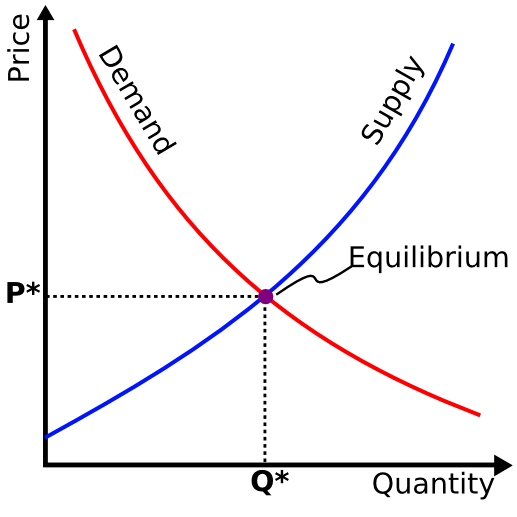
\includegraphics[scale=0.4]{supply&demand.jpg}
\caption{Equilibrium price and quantity \citep{gjerstad1998price}}
\label{fig:univerise}
\end{figure}

Before going to the Double auction modelling part,let us first discuss some basics of demand and supply curve :\citep{gjerstad1998price}\\
\noindent Laws of supply and demand:
\begin{itemize}
\item All else being equal, an increase in price results in an increase in quantity supplied.
\item All else being equal, as the price of a product increases, quantity demanded decreases.
\end{itemize}
Law of demand:
\begin{itemize}
\item Pretty robust law
\item As prices get lower, there are more possible applications/uses
\item As prices get lower, the good can be substituted for other goods
\item Exceptions:
\begin{itemize}
\item \textbf{Giffen goods:} As prices rise, less money for preferable alternatives
\item \textbf{Veblen goods:} As prices rise, the good becomes more of a status symbol
\end{itemize}
\end{itemize}
Law of supply:
\begin{itemize}
\item Much more complicated
\item Short-term vs long-term
\begin{itemize}
\item \textbf{Short-term:} Increase production at single plant, idle single plant
\item \textbf{Long-term:} Build new plants
\end{itemize}
\begin{itemize}
\item Extractive industries
\begin{itemize}
\item Easy vs difficult to extract resources
\end{itemize}
\item Efficiencies of scale
\begin{itemize}
\item With automation, making more reduces unit costs
 \item Eventually, you run out of scarce resources
\end{itemize}
\end{itemize}
\end{itemize}
\section{Regret felt by a single seller for dynamic pricing of the product}
Let us assume that V(t) is price of an item on a given time t.\\
\noindent Also, assume that there is only a single player who first has to to buy the item ,then has to sell it,ensuring some positive profit to him.\\
\noindent \textbf{Note:} Player will feel regret in a period only when,if there is no transaction (either buying or selling)in that period.
So the algorithm for finding out the regret of the player is as below:\citep{gjerstad1998price}
\begin{enumerate}
\item[\textbf{1.}] Player will always buy the product in first period,irrespective of the price.But this price must be less than or equal to player's valuation.
\item[\textbf{2.}] Player will always sell the in-hand product in last period,irrespective of the price in the last period.i.e., there should not be any inventory left with the player after the last period.
\item[\textbf{3.}] For rest of the period player will be transaction in period t if and only if,\\
$V[t]<V[t+1]\hspace*{2mm} \& \hspace*{2mm}V[t-1]<V[t]$\\
\noindent Otherwise player will fill regret in the period t.
\end{enumerate}


\section{Double Auction with Zero Intelligence (ZI) Agents \citep{dong2014double}}
Double Auction:
\begin{itemize}
\item Both buyers and sellers place bids in the auction
\item] Buyers and sellers can alter their bids as the auction proceeds
\item The auction is finished when the ask is below the bid
\item Double auctions will be thus used as model of market price finding mechanisms
\end{itemize}
Zero Intelligence Agents:
\begin{itemize}
\item Buyers bid random amount below their redemption value
\item Sellers bid random amount above their cost
\item Bids are only accepted if they actually increase the bid or decrease the ask
\end{itemize}
Below is the output of the algorithm coded in python for above algorithm:
\begin{figure}[H]
\centering
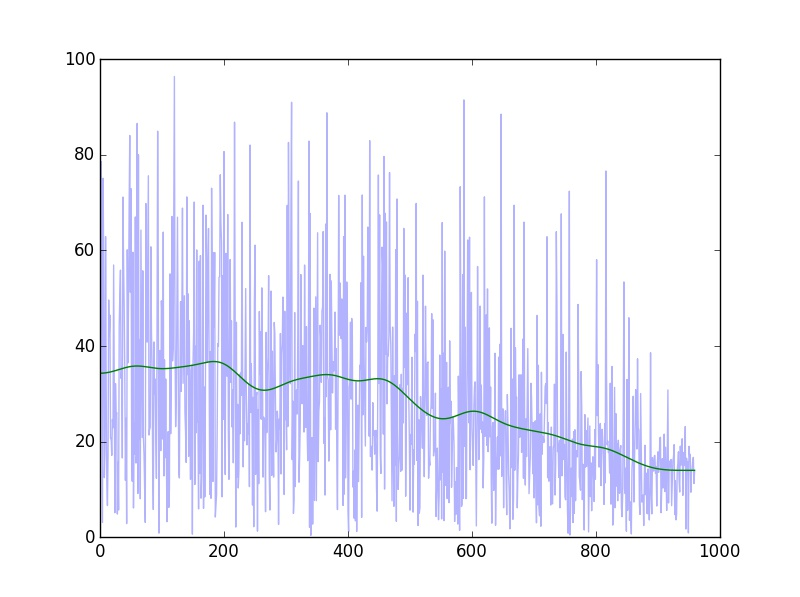
\includegraphics[scale=0.4]{figure_1.jpg}
\caption{As the double auction proceeds, prices converge towards the market clearing price \citep{gjerstad1998price}}
\label{fig:univerise}
\end{figure}

\section{Conclusion from the model}
Markets tend towards clearing prices even in the absence of intelligence as the double auction proceeds,which can be seen from \ref{fig:univerise}.\\
\noindent But conversing of clearing price depends on the following factors:
\begin{itemize}
\item Nature of demand and supply curve
\item Number of simulations
\item Probability of choosing player for their bid revision
\end{itemize}
 And, now below are the questions generated from the model regarding future work:
 \begin{enumerate}
 \item[\textbf{1.}] Does this really tell us about real market price mechanisms?
\item[\textbf{2.}] Is this more of an oddity?
\item[\textbf{3.}] What kinds of real-world markets does it describe?
\item[\textbf{4.}] A lot of buyers/sellers are paying "the wrong price", what are the implications? 
 
\end{enumerate}

\chapter{Further discussion}
We will try to see the effect of loser as well as winner regret under different types of auction also, namely Second price sealed bid, Dutch, and English auction.\citep{filizy2005auctions}
\section{Winner Regret in Other Auctions}
\subsection{Second price auction:}
Suppose the seller sells the object by a second price sealed bid auction (SP), i.e., the participants submit their bids in sealed envelopes and the highest bidder gets the object at the price of the second highest bid. Theoretically, unlike the first price, in the second price sealed bid auction, the winner will not regret her bid. In this type of auction, by changing their bids, the bidders can affect only their winning/losing positions. So, winner regret will not change the form of utility.

\subsection{Dutch auction:}
The Dutch auction is a \textbf{descending price auction} in which a public price clock starts out at a high level and falls until the first participant accepts to pay the price. In a Dutch auction, it is not possible to define the effect of winner regret because in the descending auction the winner never learns whether she would have won if she waited a bit more.

\subsection{English auction:}
The English auction is an \textbf{ascending price auction} in which bidders increase the current price, and the last remaining bidder receives the object at the amount at which no further price increases are made. Similar to SP, in an English auction, introducing \textbf{winner regret into the model does not affect the form of utility}. Obviously, in the ascending auction the winner already pays the smallest possible amount, which makes her the winner.\\[3mm]

\noindent \textbf{REMARK 5:} Since winner regret does not enter the utility in second price, English, or Dutch auctions, the optimal bidding strategy will be the same as in the traditional case. Hence, the expected revenue of the seller will be the same whether the bidders have winner regret or not. However, due to Remark 4, the expected revenue decreases in FP if the bidders have winner regret concerns.\citep{filizy2005auctions}

\noindent Thus \textbf{the expected revenue in FP is the lowest among these four auctions, and it is the same in second price, English, and Dutch auctions under winner regret concern}.

\section{Loser Regret in Other Auctions}
	\subsection{Second price auction:}
Unlike the winner regret, bidders may feel loser regret in SP because, for example, a bidder might bid less than her valuation and might learn that the winning bid is lower than her bid. This does not happen in the equilibrium, however, because truth-telling is the dominant strategy for the SP with loser regret, as in the traditional theory. So the following theory comes into picture:\\[3mm]
\textbf{THEOREM 3:} In a second price sealed bid auction with loser regret, the symmetric equilibrium bidding strategy is \citep{filizy2005auctions} \\

\noindent $b^{{SP}_{lr}}(V)= V$  

\begin{flushright}
$\forall$ $V\in [\underline{V} , \overline{V}]$\end{flushright}
\subsection{Dutch auction:}
Unlike the analysis under winner regret, this time loser regret may be felt in a Dutch auction because information on the winning bid is known. The way bidders anticipate loser regret is exactly the same as that in FP. Therefore, the same analysis done for FP applies here, and implies the same equilibrium strategy.

\subsection{English auction:}
Similar to SP, in the English auction, loser regret is not felt in equilibrium, since bidders will bid their true values, so the winning bid will not be affordable for the ones who lost the auction in the equilibrium.\\[3mm]

\noindent \textbf{REMARK 6:} Loser regret is not felt in the second price and English auctions in equilibrium, and hence the expected revenue remains the same as in the traditional case. The loser regret can, however, be felt and increases the optimal bid in comparison to the RNNE in first price and Dutch auctions, and hence it increases the expected revenue of the seller.\citep{filizy2005auctions}

\noindent Thus \textbf{if bidders have loser regret concerns, the expected revenue of the seller is higher in first price and Dutch than in second price and English auctions.}

\chapter{Conclusion $\textbf{\&}$ Future work}
Based on the whole discussion throught the report along with the experimental finding, we can conclude the results listed below:
\begin{enumerate}
\item[\textbf{1.}] Overbidding in first price auctions is derived from the anticipation of loser regret. 
\item[\textbf{2.}] Experimental results suggest that \textbf{bidders can indeed, anticipate loser regret}. On the other hand, in the experiment, \textbf{the bidders could not anticipate winner regret} and hence did not reflect these feelings in their bids.
\item[\textbf{3.}] The expected revenue in FP is the lowest among these four auctions, and it is the same in second price, English, and Dutch auctions under winner regret condition.
\item[\textbf{4.}] If bidders have loser regret concerns, the expected revenue of the seller is higher in first price and Dutch than in second price and English auctions.
\item[\textbf{5.}] Markets tend towards clearing prices even in the absence of intelligence,with the progress of double auction theory.
 \end{enumerate}
 \section{Future Work}
Below are lists of some future works (questions),which are interesting as well as challenging and uses the concept of auction (or double auction) with regret parameters:
 \begin{enumerate}
\item[\textbf{1.}] Does the model on double auction really tell us about real market price mechanisms?
\item[\textbf{2.}] Is the model derived in chapter 4 more of an oddity?
\item[\textbf{3.}] What kinds of real-world markets does the model in chapter 4 describe?
\item[\textbf{4.}] A lot of buyers/sellers are paying "the wrong price", what are the implications of it in the modelling of double auction?
\item[\textbf{5.}]What, if the distribution of valuation is not a common knowledge to every bidders (players)in double auction model?
\item[\textbf{6.}] As a player in the double auction market,what will be the probability and parameter of modelling a regret parameter,given that me as an player of enough intelligence?
\end{enumerate}
\nocite{*}
\bibliographystyle{plain}
\bibliography{Ref}

%appendix starts from here
\begin{appendix}
\chapter{Python code for Regret felt by a single seller for dynamic pricing of the product}
\begin{listing}
\label{ap_1}
\section{Code for probability of regret}
from numpy.random import *\\
import numpy as np\\ 
import matplotlib.pyplot as plt\\
%matplotlib inline
seed(123)\\
i=0\\
d=input('distribution is 1 (exponential),2(uniform),or 3(normal),or 4(unknown distribution):')\\
s=input('size is:')\\
if int(d)==1:\\
    p=input('parameter is:')\\
    V=exponential(1.0/p,s)\\
elif int(d) == 2:\\
        a=input('lower limit of parameter is:')\\
        b=input('upper limit of parameter is:')\\
        V=uniform(int(a),int(b),int(s))
elif int(d) == 3:\\
        a=input('mean of the distribution is:')\\
        b=input('std. of the distribution is:')\\
        V=normal(int(a),int(b),int(s))\\
else:\\
    V = np.random.uniform(0,1.5,s)+2*np.random.uniform(3,4,s)-(1.0/np.random.uniform(1,4,s))\\
    print list(V)\\
n=len(V)\\
count=0\\
print("buy in the period",1)\\
for i in range (1,n-1):\\
    if V[i]<V[i+1]:\\
        if V[i-1]<V[i]:\\
            count=count+1\\
            print("feel regret (i.e., No transaction) in the period", i+1)\\
        i=i+1\\
    else:\\
        print("sell in the period",i+1)\\
        print("and buy in the period",i+2)\\
print("sell in the period",s)\\
print "probability that a given seller is going to feel regret is,",float(count)/n\\

\section{Code for Distribution Verification of random data}
Import histogram function from Matplotlib\\
from matplotlib.pyplot import hist\\
% To show plots directly in the notebook\\
matplotlib inline\\
import numpy as np\\
from scipy.stats import norm\\
from scipy.stats import chisquare, chi2\\
y=list(V)\\
n=len(V) %Number of data points\\
k=n/5 %Number of intervals\\
print ("Number of data points", n)\\

\noindent Estimate Lambda as per MLE formula\\
$est_m=np.mean(y)$\\
$est_sd=np.std(y)$\\

\noindent Compute End points. Used 'List Comprehension' \\
%See http://www.secnetix.de/olli/Python/list_comprehensions.hawk for more examples\\
$endpts=[norm.ppf(float(j)/k,loc=est_m, scale=est_sd) for j in range(0,k)]$\\
print ('ed=',endpts)\\
endpts.append(max(y)+1)\\
print ('End Points of histogram', endpts)\\

\noindent h = hist(y, bins=endpts)\\
obs = h[0]\\
print ("Observed values in each bin", obs)\\

\noindent exp = float(n)/k\\
print ("Expected number in each bin", exp)\\

\noindent Perform Chi-Square Test\\
TestStat, pvalue = chisquare(obs,exp)\\
print ("Test Statistics: Chisquare =", TestStat, "  p-value=", pvalue)\\

\noindent alpha=0.05\\
%Compute the Chi-Square Distribution value for the given value of Alpha\\
print ("ChiSq Distribution value",chi2.ppf(1-alpha, k-1))\\
\end{listing}
\chapter{Python code for Double Auction with Zero Intelligence (ZI) Agents}
\label{ap_2}
\begin{listing}
\section{Code for supply and demand curve}
from array import *\\
import matplotlib.pyplot as plt\\
from numpy.random import *\\
N=input('the number of sellers(or buyers) is:')\\
seed(123)\\
costs = rand(N)**2*100.0\\      %these are the valuations for the marginal cost of all the sellers
redemptions = rand(N)**3*100.0\\ %these are the valuations for the marginal benefits of all the buyers
plt.plot(sorted(costs))\\
plt.plot((sorted(redemptions))[::-1])\\
plt.show()\\
\section{Code for calculation of clearing price}
from pylab import *\\
 calculating the clearing(market or equilibrium) price\\
nclearing = find(array(sorted(costs))>=array(sorted(redemptions))[::-1])[0]\\
print ("equilibrium quality for the market is:",nclearing)\\
clearing = sorted(costs)[nclearing]\\
print ("equilibrium price for the market is:",clearing)\\

\section{Code for initiation of double auction}
initiating the double auction process\\
sellers = set(range(N))\\
buyers = set(range(N))\\
transactions = []\\
alltrans = []\\
gain = 0\\
length=N\\
for r in range(N):\\
    ask = 100.0\\
    seller = -1\\
    bid = 0.0\\
    buyer = -1\\
    last = -999\\
    for r in range(100):\\
        if rand()<0.5:\\
            i = list(sellers)[int(floor(rand()*length))]\\ %selecting at random one seller out of N
            new ask = rand()*(100-costs[i])+costs[i]\\     %revising the ask price of the seller
           
            \begin{equation*}
            \begin{cases}
           \text{ if new ask}<\text{ask}:\\
                \text{ask} = \text{new ask}\\
                \text{last} = \text{ask}\\
            \text{seller} = \text{i}                                        
\end{cases}            
            \end{equation*} \\
        else:\\
            j = list(buyers)[int(floor(rand()*length))]\\  %selecting at random one buyer out of N
            \begin{equation*}
            \begin{cases}
            \text{new bid} = \text{rand}()*\text{redemptions[j]}             \\ %revising the bid price of the buyer
            \text{if new bid}>\text{bid:}\\
                \text{bid} = \text{new bid}\\
                \text{last} =\text{ bid}\\
                \text{buyer} = \text{j}\\
        \text{if ask}<\text{bid}:                                   
 \end{cases}        
         \end{equation*} \\ % this is the condition for transaction between buyer and seller
            sellers -= {seller}                         \\ %sellers=sellers-{seller} i.e., exclude this perticular seller from the list
            buyers -= {buyer}                           \\ %buyers=buyers-{buyer} i.e., exclude this perticular buyer from the lis
            transactions.append(last)                    \\
            assert last>=costs[seller]                  \\ % this ensures no loss to the seller. i.e., no negative payoff
            assert last<=redemptions[buyer]             \\ % this ensures no loss to the buyer. i.e., no negative payoff
            gain += (redemptions[buyer]-costs[seller])\\   %this is the maximum gain to the sellers
            length-=1\\
            break\\
print ('list of sellers who could not sell their product is:',list(sellers))\\
print ('list of buyers who could not buy the product is:',list(buyers))\\
print ('total number of transactions is:',(N-len(buyers)))\\
\end{listing}
\end{appendix}
\end{document}
